\documentclass{article}
\usepackage[utf8]{inputenc}
\usepackage[spanish]{babel}
\usepackage{graphicx}
\usepackage{dirtytalk}
\usepackage{caratula}
\usepackage{enumerate}
\usepackage{amssymb}
\usepackage{algorithm}
\usepackage{algpseudocode}
\usepackage{amsmath}
\usepackage{amsthm}
\usepackage{float}
\usepackage{geometry}
\usepackage{fixltx2e}
\usepackage{wrapfig}
\usepackage{cite}
\usepackage{ dsfont }
\usepackage{float}
\usepackage[space]{grffile}
\usepackage{tpalgo3}
\geometry{
 a4paper,
 total={210mm,297mm},
 left=30mm,
 right=30mm,
 top=30mm,
 bottom=30mm,
 }
 
\newtheorem{theorem}{Teorema}[section]
\newtheorem{corollary}{Corolario}[theorem]
\newtheorem{lemma}{Lema}[theorem]
 
\theoremstyle{definition}
\newtheorem{definition}{Definición}[section]
 
\theoremstyle{remark}
\newtheorem*{remark}{Observación}
 
\begin{document}
% Estos comandos deben ir antes del \maketitle
\materia{Algorítmos y Estructuras de Datos III} % obligatorio

\titulo{Trabajo Práctico 1}
\subtitulo{}
\grupo{}

\integrante{Bayardo Julián}{850/13}{julian@bayardo.com.ar} % obligatorio
\integrante{Cuneo Christian}{755/13}{chriscuneo93@gmail.com} % obligatorio 
\integrante{Frassia Fernando}{340/13}{ferfrassia@gmail.com} % obligatorio 
\integrante{Gambaccini Ezequiel}{715/13}{ezequiel.gambaccini@gmail.com} % obligatorio 
 
\maketitle

\pagebreak

\tableofcontents

\pagebreak

\section{Problema 1}

\subsection{Enunciado}
La comunicación es el progreso! decididos a entrar de lleno en la nueva era el país decidió conectar telegráficamente todas las estaciones del moderno sistema férreo que recorre el país en abanico con origen en la capital (el kilómetro 0). Por lo escaso del presupuesto, se ha decidido ofrecer cierta cantidad de kilómetros de cable a cada ramal. Pero para maximizar el impacto en épocas electorales se busca lograr conectar la mayor cantidad de ciudades con los metros asignados (sin hacer cortes en el cable).
Resolver cuantas ciudades se pueden conectar para cada ramal en $O(n)$ , con n la cantidad de estaciones en cada ramal, y justificar por qué el procedimiento desarrollado resuelve efectivamente el problema.

\subsection{Breve descripción del algoritmo}

Para resolver este problema, colocamos los kilometrajes de las ciudades en una lista, luego creamos cuatro variables para recordar el comienzo y fin del camino actual, y el comienzo y fin del mejor camino (en este caso, el que incluye a la mayor cantidad de ciudades). \\
Al ir recorriendo la lista de ciudades, mientras que podamos avanzar nuestro fin de camino actual sin pasarnos de la cantidad de metros disponibles a utilizar, avanzamos el fin, y si por el contrario, no podemos avanzar más debido a que excederíamos la cantidad de metros disponibles, avanzamos el principio del camino actual (para recuperar metros disponibles) hasta que podamos avanzar (porque tenemos más metros disponibles de los que requiere conectar la siguiente ciudad, o porque ni con todos los disponibles posibles podemos hacerlo, con lo cual dejamos el inicio y el fin en esta ciudad, y avanzamos). \\
En cada iteración, comparamos la cantidad de ciudades acumuladas en el camino actual contra las acumuladas en el mejor camino, y de ser el caso, lo actualizamos. \\
Finalmente, obtenemos las posiciones donde se inicia y se termina el mejor camino, y devolvemos la diferencia entre sus índices + 1. \\

\nuevoAlgo{Algoritmo 1}{maxCantDeCiudades($meters$: $Nat$, $distances$: $Vector<Nat>$)} $\rightarrow$ $res$ :
$Nat$ \\ 
Dado un natural (Meters) y una lista de distancias entre ciudades (Distances), devuelve la cantidad máxima de ciudades que se pueden recorrer con esta cantidad de metros. \\ 

\begin{algorithmic}[1]
\State \textbf{\textit{maxCantDeCiudades:}} $meters: Nat, distances: Vector<Nat>$
\State $bestStart\gets 0$\Comment{$O(1)$}
\State $bestEnd\gets 0$\Comment{$O(1)$}
\State $start\gets 0$\Comment{$O(1)$}
\State $end\gets 0$\Comment{$O(1)$}
\State \textbf{\textit{mientras}} $end < tamano(distances)$
%\For {$end = 0$ , $end < tamaño(distances)$ , $end = end + 1$}
\State \qquad \textbf{\textit{mientras}} $distances[end] - distances[start] > meters$
\State \qquad \qquad start++\Comment{$O(1)$}
\State \qquad \textbf{\textit{si}} {end - start $>$ bestEnd - bestStart}\Comment{$O(1)$}
\State \qquad \qquad bestStart $\gets$ start\Comment{$O(1)$}
\State \qquad \qquad bestEnd $\gets$ end\Comment{$O(1)$}
\State $end\gets end + 1$\Comment{$O(1)$}
%\EndFor
\State $output \gets 0$\Comment{$O(1)$}
\State \textbf{\textit{si}} bestStart $\neq$ bestEnd\Comment{$O(1)$}
\State \qquad output $\gets$ bestEnd - bestStart + 1\Comment{$O(1)$}
\State \textbf{return} output
\end{algorithmic}


\subsection{Correctitud}
Para convencernos de que nuestro algoritmo es correcto, veamos cómo funciona el mismo, y por qué la solución que se obtiene de él es una solución al problema. \\ 
Para esto, debemos ver que: 
\begin{enumerate}
\item Primero, que estamos armando correctamente el camino parcial, es decir, que la suma de las distancias entre las ciudades del camino es menor que la cantidad de metros disponible y además es el más largo de los que tienen como última ciudad a la ciudad actual (es decir, no existe una ciudad anterior a la del principio del camino, tal que siga siendo un camino válido).
\item Segundo, que en cada iteración, nos quedamos con un camino válido más largo desde la primera ciudad hasta la ciudad iterada.
\item Tercero, que habiendo encontrado uno de los caminos más largos, devolvemos su longitud.
\end{enumerate}

1. Con respecto al primer punto, veamos que cada vez que iteramos por una ciudad, nos preguntamos si podemos anexarla a nuestro camino de acuerdo a la cantidad de metros que tenemos y la 'longitud' del camino. Y de no ser posible anexarla, recortamos el principio (de a una ciudad por vez) hasta llegar a una 'longitud' que sí nos permita anexarla. No está de más aclarar que buscamos el mínimo recorte de camino posible, y es por eso que en cada "recorte" nos preguntamos si en ese instante podemos anexarla. Habiendo dicho esto, podemos decir que para cada ciudad, la estamos incluyendo en un camino parcial válido, y además es el máximo de los caminos actuales que podemos formar con esa ciudad como fin. \\

Demostrémoslo formalmente: \\

Sea V = $\{\mathcal{V}_1,..., \mathcal{V}_n\}$ una secuencia de n ciudades, sea m la cantidad de kilómetros de cable para conectarlas y sea V'$_{ij}$ = $\{\mathcal{V}_i,..., \mathcal{V}_j\}$ con i,j $\in$ $\{1..n\}$, i $\leq$ j, una subsecuencia válida (es decir, V' es una subsecuencia válida de V si y sólo si $\mathcal{V}_j$ - $\mathcal{V}_i$ $\leq$ m $\wedge$ $\nexists$ 1 $\leq$ i' $<$ i $/$ $\mathcal{V}_j$ - $\mathcal{V}_{i'}$ $\leq$ m). \\

Quiero ver que $\forall$ j $\in$ $\{1..n\}$, en la j-ésima iteración, el algoritmo elige i tal que la subsecuencia $\mathcal{V}_{ij}$ es válida.\\

\textbf{\textit{Inducción:}} \\

P(j) = $\forall$ j $\in$ $\{1..n\}$ en la j-ésima iteración el algoritmo elige i $/$ \\
a) $\mathcal{V}_j$ -  $\mathcal{V}_i$ $\leq$ m $\wedge$ \\
b) $\nexists$ 1 $\leq$ i' $<$ i $/$ $\mathcal{V}_j$ - $\mathcal{V}_{i'}$ $\leq$ m \\

\textit{Caso Base:} \\
P(1) = En la primera iteración, el algoritmo elige i $/$ $\mathcal{V}_j$ - $\mathcal{V}_i$ $\leq$ m \\

a) Notemos que no se cumple la guarda del primer condicional, dado que $end(j)$ y $start(i)$ son ambos la primera posición de la secuencia V. Entonces, como i = j, $\mathcal{V}_j$ -  $\mathcal{V}_i$ = 0, que es siempre menor o igual a m, por ser m una distancia. \\

b) Dado que i es la primera posición de la secuencia, es decir, como i = 1, no existe un i' mayor o igual a 1 y menor estricto que 1 a la vez, con lo cual vale c.\\

\textit{Paso Inductivo:} \\
Quiero ver que $\forall$ j $\in$ $\{2..n\}$, P(j - 1) $\Rightarrow$ P(j) \\ 
Hipótesis Inductiva: Vale P(j - 1), es decir, vale que para la j-1-ésima iteración, el algoritmo eligió i $/$ \\
a) $\mathcal{V}_{j-1}$ - $\mathcal{V}_i$ $\leq$ m $\wedge$ \\
b) $\nexists$ 1 $\leq$ i' $<$ i $/$ $\mathcal{V}_{j-1}$ - $\mathcal{V}_{i'}$ $\leq$ m \\

Como acabo de cubrir una nueva ciudad, tengo que ver los casos en que:\\
1) $\mathcal{V}_j$ - $\mathcal{V}_i$ $\leq$ m \\
2) $\mathcal{V}_j$ - $\mathcal{V}_i$ $>$ m \\

CASO 1): $\mathcal{V}_j$ - $\mathcal{V}_i$ $\leq$ m \\
a) Dado que estoy en el caso 1, vale.\\
b) Sé que $\nexists$ 1 $\leq$ i' $<$ i $/$ $\mathcal{V}_{j-1}$ - $\mathcal{V}_{i'}$ $\leq$ m (por HI), quiero ver que $\nexists$ 1 $\leq$ i' $<$ i $/$ $\mathcal{V}_j$ - $\mathcal{V}_{i'}$ $\leq$ m \\

Veamos por el absurdo: \\
Sé que $\forall$ j $\in$ \{2..n\} vale que $\mathcal{V}_{j-1}$ $<$ $\mathcal{V}_j$, por orden creciente estricto. \\
Si existiera 1 $\leq$ i' $<$ i $/$ $\mathcal{V}_j$ - $\mathcal{V}_{i'}$ $\leq$ m \\
significaría que:  $\mathcal{V}_{j-1}$ - $\mathcal{V}_{i'}$ $<$ $\mathcal{V}_j$ - $\mathcal{V}_{i'}$ $\leq$ m \\
entonces: $\mathcal{V}_{j-1}$ - $\mathcal{V}_{i'}$ $\leq$ m   ABS! \\
es absurdo porque por hipótesis inductiva sabíamos que no existía i' que cumpliera con eso. \\

CASO 2): $\mathcal{V}_j$ - $\mathcal{V}_i$ $>$ m \\
a) Dado que la secuencia está ordenada de forma estrictamente creciente y que mientras $\mathcal{V}_j$ - $\mathcal{V}_i$ sea mayor estricto que m el algoritmo aumenta i en una unidad, $\mathcal{V}_j$ - $\mathcal{V}_i$ va reduciéndose hasta ser menor o igual a m, donde i se detiene y el ciclo termina. Esto sucede de una de dos formas: \\

O bien $\exists$ 1 $\leq$ i' $<$ i'' $/$ $\mathcal{V}_j$ - $\mathcal{V}_{i''}$ $\leq$ m \\
en cuyo caso se obtiene que i pasa a valer i'', y se cumple a).

O bien $\nexists$ 1 $\leq$ i' $<$ i'' $/$ $\mathcal{V}_j$ - $\mathcal{V}_{i''}$ $\leq$ m \\
en cuyo caso, al llegar i = j, $\mathcal{V}_j$ - $\mathcal{V}_i$ = 0, lo cuál es menor o igual a m, por ser m una distancia. \\

b) Ídem al b) del CASO 1.\\

Ahora sabemos que los caminos generados en cada iteración son válidos, pero lo que nos falta probar es que en cada iteración, nos quedamos con el más largo de todos hasta el momento. \\

Por caso 1 y caso 2, vale el paso inductivo. Luego, como probamos el caso base y el paso inductivo: vale P(j) \\

2. Con respecto al segundo aspecto, en cada iteración, estamos comparando la longitud del camino actual contra la longitud del camino parcial histórico, y actualizándolo según quién sea más largo. Entonces, como el camino parcial histórico era uno de los más largos hasta el momento, y ahora al compararlo obtenemos un nuevo camino parcial histórico podemos asegurar que en la ciudad iterada obtenemos uno de los caminos parciales históricos más largos. \\

Demostrémoslo formalmente: \\

Quiero ver que $\forall$ j $\in$ \{1..n\}, en la j-ésima iteración, el algoritmo se queda con uno de los caminos válidos más largos hasta j. \\

\textbf{\textit{Inducción: }} \\

P(j) = en la j-ésima iteración, el algoritmo se queda con uno de los caminos válidos más largos hasta j. \\

\textit{Caso Base:} \\
P(1) = No hay camino válido con una sola ciudad, con lo cual me quedo con el camino válido nulo, que siendo el único, es el más largo. \\

\textit{Paso Inductivo:} \\
Quiero ver que $\forall$ j $\in$ \{2..n\}, P(j - 1) $\Rightarrow$ P(j) \\
Hipótesis Inductiva: Vale P(j - 1), es decir, para la j-1-ésima iteración, el camino parcial histórico es uno de los caminos más largos hasta j-1. \\

Quedan dos casos a evaluar en la iteración j: \\
CASO 1: \\
$\vert$camino(j)$\vert$ $\leq$ $\vert$camino histórico(j-1)$\vert$ \\
CASO 2: \\
$\vert$camino(j)$\vert$ $>$ $\vert$camino histórico(j-1)$\vert$ \\

CASO 1:
Como el $\vert$camino(j)$\vert$ es menor o igual al histórico de j - 1, no modificamos el camino guardado hasta el momento, y como sabíamos que valía P(j-1), es decir que era uno de los caminos más largos hasta j - 1, vale que es uno de los caminos más largos hasta j. Osea, vale P(j). \\

CASO 2:
Acá se cumple la guarda del condicional y nos quedamos con el camino(j). Y como por HI valía que el camino histórico era uno de los más largos hasta j - 1, y en j encontramos uno más largo que ese, entonces vale que en particular el camino j es uno de los más largos hasta j. \\

Por caso 1 y caso 2, vale el paso inductivo. Luego, como probamos el caso base y el paso inductivo: vale P(j) \\

Por ambas demostraciones, probamos que el algoritmo genera un camino válido en cada iteración, y además se queda con el más largo hasta el momento. \\

3. Finalmente, se demuestra trivialmente que el algoritmo devuelve la longitud del camino encontrado.


\subsection{Complejidad}
Como el algoritmo descripto es el único utilizado en la resolución del problema, y como pueden apreciarse las complejidades de las operaciones en el pseudocódigo, lo único que queda por analizar son los ciclos que contiene. \\
Se puede ver que el algoritmo contiene un ciclo principal, el cual siempre realizará tamaño$(distancia)$ iteraciones. Luego, dentro de este ciclo hay otro ciclo y un condicional, el cuál ignoraremos porque que toma tiempo constante. Finalmente veremos cuál es la complejidad del ciclo secundario, y concluiremos que en peor caso, la complejidad del ciclo principal es $O(\text{tamaño}(distancia))$. \\ 
Primero tomemos el caso en que, en cada iteración se cumple la guarda del ciclo .
Como podemos ver, el ciclo chequea que:
\begin{enumerate}
\item Es posible cubrir la sub-secuencia actual de ciudades con el cable dado, puesto que éste es más largo.
\end{enumerate}

Veamos que si la condición del ciclo se cumple en cada iteración del ciclo principal, eso significa que la cantidad de metros de cable es menor a toda distancia entre cualquier par de ciudades, y más aún, esto también vale para todo par de ciudades adyacentes. Con lo cual, en cada iteración del ciclo principal, el ciclo secundario se ejecutará una sola vez, y luego se romperá su guarda. Esto es porque cada vez que se aumenta $end$, se cumple la guarda del ciclo secundario, con lo cuál aumenta $start$, luego $start$ y $end$ valen lo mismo, y por eso se rompe la guarda. Habiendo dicho esto, podemos ver que: dado que el ciclo secundario se ejecuta una sola vez, y que cada ejecución del mismo cuesta $O(1)$, el ciclo mismo cuesta $O(1)$; con lo cual el ciclo principal cuesta $O(\text{tamaño}(distancia))$.

Veamos otro caso, en el que el ciclo secundario puede ser más costoso. \\
Tomemos el caso en el que el ciclo itera la mayor cantidad de veces posible (dado que la instrucción dentro del mismo es constante, y no hace falta tomarla en cuenta). Notemos que esto sucede cuando $start$ y $end$ están lo más distanciados posible, y además se cumple que la diferencia entre ellos es mayor a los metros de cable. Es claro que esto se da cuando $start$ es la primera ciudad, y $end$ es la última, y además la diferencia entre la última ciudad y la ante-última es más grande que la cantidad de metros de cable (esto fuerza a que necesariamente el ciclo itere hasta que $start$ sea igual a $end$). En este caso podemos ver que el ciclo secundario itera $\text{tamaño}(distancia)$ veces, pero veamos que en todas las iteraciones del ciclo principal necesariamente ésta es la primera y única vez que se ejecuta este ciclo secundario. Esto es porque asumimos que $start$ debía estar al principio, y por eso es que el ciclo secundario no podría haberse ejecutado hasta este momento. Con lo cual vemos que para todas las iteraciones del ciclo principal exceptuando la última, el ciclo toma $O(1)$ y en la última toma $O(\text{tamaño}(distancia))$. Entonces se tiene que la complejidad es $O(\text{tamaño}(distancia) - 1)$ + $O(\text{tamaño}(distancia))$ = $O(\text{tamaño}(distancia))$ \\
Finalmente, todos los demás casos estarán entre medio de estos dos. Es decir, entre correr en todas las iteraciones del ciclo principal con costo $O(1)$, y correr una sola vez con costo $O(\text{tamaño}(distancia))$. Y por eso podemos decir que el costo del algoritmo en peor caso es $O(\text{tamaño}(distancia))$.


%La primera condición es mas débil que la segunda, por lo tanto va a volverse $falsa$ antes o al mismo tiempo que la segunda sin excepción. Por lo tanto podemos descartarla a la hora de analizar la cota superior de complejidad. 
%La segunda condición va a volverse $falsa$ en el momento que $start$ sea igual a $end$, ya que en cualquier estado del programa al que se pueda llegar desde el estado inicial, $start$ nunca sera mayor a $end$.
%Lo importante de esta condición, al contemplarse dentro del contexto en el que se encuentra, es que, como $end$ siempre incrementa en 1 en cada iteración del $for$ y $start$ nunca decrementa, e incrementa solo cuando se haga una iteración de este ciclo $while$, y como este se ingresa a este ciclo solo mientras $start < end$, este ciclo solo hará $tamaño(distance)$ iteraciones en toda la ejecucion de este algoritmo, ya que $tamaño(distance)$ es el valor máximo que puede tomar $end$ y por lo tanto también $start$.

%Por lo tanto, teniendo en cuenta que todas las operaciones realizadas además de los ciclos son operaciones básicas con complejidad uniforme $\theta(1)$, todo el algoritmo pertenece a $O(\text{tamaño}(distances))$

\subsection{Análisis}

Al analizar este caso se nos presento el problema de que, al pertenecer a una complejidad del orden lineal, y al ser tan simple el algoritmo, no hay un peor caso "real" que se pueda analizar profundamente. Lo que queremos ver es si, en distintos casos con la misma cantidad de ciudades, el tiempo de computo del algoritmo se puede ver afectado ya sea por una distribución de distancias especificas junto a una longitud de cable especifica.
Como se puede ver en el pseudocodigo, el ciclo principal del algoritmo va a realizar exactamente una iteración por ciudad que haya en el vector de entrada, por lo tanto no se vera afectada por ningún caso especifico. Donde si podremos notar cambios es dentro de este ciclo, ya que encontraremos:
\begin{itemize}
\item un ciclo condicional
\item un bloque condiciona
\end{itemize}
El primero, como vimos en el análisis de complejidad, realizara $\text{tamaño}(distances)$ iteraciones como máximo en toda la ejecución del algoritmo, por lo tanto un peor caso seria en el cual todas estas iteraciones se realicen, y hay muchas formas de que esto suceda, la mas simple es que la ultima ciudad se encuentre a mas de $meters$ distancia de la anteutima ciudad, en ese caso al llegar a la ultima estación el algoritmo ingresara a este ciclo y realizara las $\text{tamaño}(distances)$ iteraciones. Otra forma seria que todas las estaciones se encuentren a mas de $meters$ distancia de su anterior, y por lo tanto en cada iteración del ciclo principal se realizara una iteración del ciclo interno.
Luego, el segundo, el bloque condicional, se ingresara solo si, en la iteración actual, el mejor camino obtenido hasta la iteración anterior junto con la ciudad actual forman un nuevo mejor camino (es decir, suman una mayor cantidad de ciudades mientras entran en la longitud del cable). Por lo tanto una entrada para la cual se busque entrar siempre en este bloque seria una en la cual la solución incluya a todas la ciudades, ya que en todas las iteraciones se actualizara el mejor camino para incluir una nueva ciudad.\par
Una forma de complementar estos peores casos específicos seria lograr que se ingrese en el bloque condicional en la mayoría de las iteraciones, y que al mismo tiempo se realicen todas las iteraciones posibles del ciclo secundario. Una forma seria un caso en el que el mejor camino incluya a las ciudades desde la capital hasta la anteultima ciudad, y la ultima ciudad este a mas de $meters$ distancia de la anteultima, logrando en este caso:
\begin{itemize}
\item Ingresar $\text{tamaño}(distances)-1$ veces a al bloque condicional
\item Relizar las $\text{tamaño}(distances)$ iteraciones disponibles del ciclo secundario.
\end{itemize}
\newline
El mejor caso seria buscar lo contrario a lo anterior, minimizar la cantidad de veces en las que se ingresa al bloque condicional y al ciclo secundario. Pero es importante ver que no se puede evitar entrar en alguna de las dos partes, ya que si el $start$ no es aumentado por el ciclo secundario entonces, ya que el $end$ aumenta por el ciclo principal, el camino incluirá mas ciudades, y por lo tanto sera mejor y se entrara en el bloque condicional para actualizar el mejor camino. Por lo tanto necesitaremos elegir cual de los dos bloques costara menos realizar, si el ciclo o el condicional. En este caso, a simple vista se ve que el ciclo solo realiza una asignación, mientras que el condicional realiza dos. Por lo tanto lo mejor sera entrar siempre en el ciclo y realizar una iteración. Entonces el mejor caso se dará en el que todas las ciudades estén a mas de $meters$ distancia de la anterior.

\section{Problema 2}

\subsection{Enunciado}

La mediana de un conjunto ordenado de $n$ números se define como $x_{(n+1)/2}$ si $n$ es impar, o como $(x_{n/2} + x_{(n/2)+1})/2$ si $n$ es par. Dados $n$ números enteros en cualquier orden se deben devolver otros $n$ números, donde el i-ésimo de ellos represente la parte entera de la mediana de los primeros $i$ números de la entrada.
Resolver en una complejidad estrictamente mejor que $O(n^2)$ donde $n$ es el número total de enteros de entrada.

\subsection{Breve descripción del algoritmo}

En este problema decidimos insertar uno por uno los elementos de entrada en una estructura especifica tal que los elementos queden ordenados y los datos necesarios para calcular la mediana se encuentren siempre a mano. Para esto decidimos utilizar un max-heap y un min-heap. Al ingresar nuevos elementos a nuestra estructura se va a hacer de forma tal que la cantidad de elementos que tiene cada heap difieran a lo sumo en 1, y que la cabeza del max-heap sea menor a la cabeza del min-heap. En otras palabras, el conjunto de elementos estará dividido en dos, quedando los elementos mas pequeños en el max-heap, y los mas grandes en el min-heap.

La elección de estructuras nos asegura que, luego de cada inserción, los elementos necesarios para calcular la mediana de los elementos vistos hasta el momento se encuentran en las cabezas de los heaps, que podemos obtener en $O(1)$.

Sabiendo que la inserción en un heap cuesta $O(\log(n))$ siendo $n$ la cantidad de elementos en el heap, al igual que eliminar la cabeza. Nuestro algoritmo insertará todos los elementos de entrada en el heap que corresponda, que serán siempre de tamaño como mucho $\frac{n}{2}$, este proceso provocara como mucho dos inserciones en heap y una quita de cabeza para mantener el invariante de la estructura (se vera mas claramente en el algoritmo).

\subsection{Correctitud}

Consideramos a los conjuntos que vamos a usar como conjuntos que aceptan repeticiones, y definimos las siguientes funciones:

\newcommand{\twopartdef}[4]
{
	\left\{
		\begin{array}{ll}
			#1 & \mbox{if } #2 \\
			#3 & \mbox{if } #4 \\
		\end{array}
	\right.
}

\newcommand{\fourpartdef}[8]
{
	\left\{
		\begin{array}{ll}
			#1 & \mbox{if } #2 \\
			#3 & \mbox{if } #4 \\
			#5 & \mbox{if } #6 \\
			#7 & \mbox{if } #8 \\
		\end{array}
	\right.
}

    Min: $C \rightarrow \mathds{Z} , \  C \subseteq \mathds{Z} $  
    
    Min(C) = $\twopartdef{ \{x / x \in C  \wedge \forall y \in C, x \leq y\} }{\#C > 0}{\infty}{\#C = 0}$ \\ \\

    Max: $C \rightarrow \mathds{Z} , \  C \subseteq \mathds{Z} $ 
    
    Max(C) = $\{x / x \in C  \wedge \forall y \in C, x \geq y\}$ \\ \\

    Mediana: $L \  \times\  R \  \rightarrow \mathds{Z}, \ L \subseteq \mathds{Z}, \ R \subseteq \mathds{Z}$
    
    Sujeto a:  $\#L > 0  \wedge  (1 \geq \#L - \#R \geq 0) \wedge ((\#R > 0 \wedge \#L > 0) \rightarrow \forall x \in L \forall y \in R (x \leq y) )$ \\ 
    
    Mediana(L, R) = $\twopartdef { \frac{Max(L) + Min(R)}{2} } {\#L = \#R} {Max(L)} {\#L \neq \#R}$\\ \\

    
    
    Agregar: $L\ \times R\ \times\ \mathds{Z}\ \rightarrow L'\  \times\  R', L \subseteq \mathds{Z}, \ R \subseteq \mathds{Z}, \ L' \subseteq \mathds{Z}, \ R' \subseteq \mathds{Z}, \ $\\
    
    Agregar(L, R, x) = $\fourpartdef { L  \ \cup \{x\}, R} 
                                    {\#L = \#R   \wedge \ \text{Min}(R) \geq x} 
                                    { L  \ \cup \{Min(R)\}, (R - \{Min(R)\}) \cup \{x\}}
                                    { \#L > 0  \wedge \ \#L = \#R \wedge \text{Min}(R) < x}
                                    {L, R \ \cup \{x\}}
                                    {\#L > 0  \wedge \ \#L \neq \#R \wedge \text{Max}(L) < x}
                                    {(L - Max(L)) \ \cup \{x\}, R \ \cup \{Max(L)\} }
                                    {\#L > 0  \wedge \ \#L \neq \#R \wedge \text{Max}(L) \geq x}$\\
      \\
          
\textbf{Predicado Inductivo}: Sea N = \#L + \#R. Mediana(Agregar(L, R, x)) devuelve la mediana de un conjunto ordenado resultado  de ${L} \cup {R} \cup {x}$. Además, $\#L > 0  \wedge  (1 \geq \#L - \#R \geq 0) \wedge ((\#R > 0 \wedge \#L > 0) \rightarrow \forall x \in L \forall y \in R (x \leq y) )$ \\ 
    


\textbf{Caso Base N = 0} \\

L = \{\} \\  

R = \{\} \\ 

Agrego un elemento x, x $\in \mathds{Z}$ \\ \\

Mediana(Agregar(L, R, x)) = 
Mediana(Agregar(\{\}, \{\}, x)) =
Mediana(\{\} $\cup$ \{x\}, \{\}) $\rightarrow$ \\ 
\#(\{\} $\cup$ \{x\}) = 1 $>$ 0 = \#(\{\}) $\rightarrow$
Mediana(\{x\}, \{\}) = Max(\{x\}) = x $\rightarrow$ x es la mediana por ser único elemento

\textbf{Paso Inductivo} \\

Supongo que es verdadero para N, N $>$ 1, analizo para N+1.\\

Hay que analizar para el caso que \#L + \#R = N sea par y para el caso que sea impar. \\

Por hipótesis inductiva, ambos conjuntos cumplen la siguiente condición para ambos casos de N (par e impar): 

(1 $\geq$ \#L - \#R $\geq$ 0) $\wedge$ ((\#R $>$ 0 $\wedge$ \#L $>$ 0) $\rightarrow$ $\forall$ x $\in$ L $\forall$ y $\in$ R (x $\leq$ y) ) \\

\textbf{Caso N Par}\\ 

Si N es par $\rightarrow$ \#L = \#R = N/2 $\wedge$ N $>$ 1.\\ 

x $\in \mathds{Z}$ \\

Mediana(Agregar(L, R, x)) $\rightarrow \twopartdef{ a) Mediana(L \ \cup \{x\}, R)}
                                                        {x \ \leq Min(R)}
                                                    {b) Mediana(L  \ \cup \{Min(R)\}, (R - \{Min(R)\}) \cup \{x\})}
                                                        {x > Min(R)}$\\
                                                        
\underline{Caso a}\\

Defino L' = L $\ \cup$ \{x\}.\\

Como x $\leq$ Min(R), L' sigue cumpliendo la precondición de mediana, ya que \#L' = 1 + N/2, \\ \#R = N/2, su diferencia es 1, y además $\forall$ x $\in$ L', $\forall$ y $\in$ R, x $\leq$ y. \\
Si L' $\cup$ R fuese un arreglo ordenado de números, su cardinal sería $1 + 2 * \frac{N}{2} = N + 1 \equiv 1 \mod 2$, por lo que la mediana sería el elemento $1 + \frac{N}{2}$ de ese arreglo. \\
Como \#L' = $1 + \frac{N}{2}$, y todos sus elementos son menores a los elementos de R, es decir, L' es la mitad más chica de un arreglo de longitud impar, teniendo L' de longitud $1 + \frac{N}{2}$, y el arreglo longitud N, la mediana debe ser el elemento más grande de este conjunto, ya que el máximo de L' es equivalente al elemento $1 + \frac{N}{2}$ del arreglo ordenado de L' $\cup$ R $\rightarrow$ Mediana(L', R) = Max(L'), que es lo que devuelve Mediana(L', R) para este caso, como queríamos demostrar.\\

\underline{Caso b}\\

Defino L' = L $\cup$ \{Min(R)\}.  \#L' = 1 + N/2 . \\

Defino R' = (R - \{Min(R)\}) $\cup$ \{x\}. \#R' = N/2 - 1 + 1 = N/2. \\

Como x $>$ Min(R), y como \#L = \#R, para mantener la precondición de Mediana, hay que extraer el mínimo de R para luego agregar x y así evitar que \#R $>$ \#L, por eso la definición anterior de R'. Luego, el mínimo extraído de R se agrega a L, quedando así definido R'. \\
De esta manera, L' y R' respetan la precondición de Mediana, ya que \\ \#L' = 1 + N/2, \#R' = N/2 $\rightarrow$ \#L' - \#R'= 1, y además, $\forall$ x $\in$ L', $\forall$ y $\in$ R', x $\leq$ y. \\
Si L' $\cup$ R' fuese un arreglo ordenado de números, su cardinal sería $1 + 2 * \frac{N}{2} = N + 1 \equiv 1 \mod 2$, por lo que la mediana sería el elemento $1 + \frac{N}{2}$ de ese arreglo. \\
Por cumplir con la precondición de Mediana, L' es la mitad más chica de un arreglo de longitud impar, teniendo L' de longitud $1 + \frac{N}{2}$, y el arreglo longitud N, la mediana debe ser el elemento más grande de este conjunto, ya que el máximo de L' es equivalente al elemento $1 + \frac{N}{2}$ del arreglo ordenado de L' $\cup$ R' $\rightarrow$ Mediana(L', R') = Max(L'), que es lo que devuelve Mediana(L', R') para este caso, como queríamos demostrar.\\

\textbf{Caso N Impar} \\ 

Si N es impar $\rightarrow$ \#L = 1 + N/2, \#R = N/2 $\wedge$ N $>$ 1.\\ 

x $\in \mathds{Z}$ \\

Como $\#L \neq \#R$: \\

Mediana(Agregar(L, R, x)) $\rightarrow \twopartdef{c) L, R \ \cup \{x\}}
                                    {Max(L) < x}
                                    {d) (L - \{Max(L)\}) \ \cup \{x\}, R \ \cup \{Max(L)\} }
                                    {Max(L) \geq x}$\\
                                    
\underline{Caso c} \\

Defino R' = R $\cup$ \{x\}. \\

Por hipótesis inductiva, \#L = 1 + N/2 y \#R = N/2. Como x $>$ Max(L), y \#R $<$ \#L, se puede definir R' sin romper la precondición de Mediana.
Si L $\cup$ R' fuese un arreglo ordenado, su longitud sería $1 + 2 * \frac{N}{2} = N + 1 \equiv 0 \mod 2$, ya que \#L = 1 + N/2 = \#R', su mediana sería el promedio entre los elementos $\frac{N+1}{2}$ y $\frac{N+1}{2} + 1$, L sería la mitad con los menores elementos del arreglo, y R' sería la mitad con los mayores elementos del arreglo $\rightarrow$ el elemento $\frac{N+1}{2}$ es el máximo de L y el elemento $\frac{N+1}{2} + 1$ es el mínimo de R'$\rightarrow$ $Mediana(L, R') = \frac{Max(L) + Min(R')}{2}$, como se quería probar. \\

\underline{Caso d} \\

Defino L'= (L - \{Max(L)\}) $\ \cup$ \{x\}, \#L'= 1 + N/2 - 1 + 1 = 1 + N/2. \\

Defino R' = R $\ \cup$ \{Max(L)\}, \#R'= 1 + N/2. \\

Como x $\leq$ Max(L), se debería redefinir L como L'= L $\cup$ \{x\}, pero esto rompería la precondición de mediana, ya que \#L' - \#R = 2 $>$ 1, por lo que L' = (L - \{Max(L)\}) $\ \cup$ \{x\}, y se redefine R como R' = R $\ \cup$ \{Max(L)\}. De esta manera, \#L'- \#R' = 0, y además, $\forall$ x $\in$ L', $\forall$ y $\in$ R', x $\leq$ y. \\
Si L' $\cup$ R' fuese un arreglo ordenado, su longitud sería $1 + 2 * \frac{N}{2} = N + 1 \equiv 0 \mod 2$, ya que \#L' = 1 + N/2 = \#R', su mediana sería el promedio entre los elementos $\frac{N+1}{2}$ y $\frac{N+1}{2} + 1$, L' sería la mitad con los menores elementos del arreglo, y R' sería la mitad con los mayores elementos del arreglo $\rightarrow$ el elemento $\frac{N+1}{2}$ es el máximo de L' y el elemento $\frac{N+1}{2} + 1$ es el mínimo de R'$\rightarrow$ $Mediana(L', R') = \frac{Max(L') + Min(R')}{2}$, como se quería probar. \\

Finalmente, de los casos N par e impar y de los subcasos a, b, c, y d, se demuestra que 
Mediana(L, R) devuelve la mediana de un conjunto ordenado resultado de la unión de L y R, cumpliendo L y R con la condición de que $1 \ \geq (\#L - \#R) \ \geq 0 \ \wedge \ ((\#R > 0 \wedge \#L >0) \rightarrow \forall x \in L \ \forall y \in R \ (x \leq y))$

\subsection{Complejidad}

Definimos una estructura Median = (left: max-heap$<$int$>$, right: min-heap$<$int$>$, output: list$<$int$>$), junto con las siguientes funciones:

\begin{algorithmic}
\Procedure{get}{m: Median}
\If{tamaño(m.left) = tamaño(m.right)}\Comment{$O(1)$}
\State \textbf{return} (top(m.left) + top(m.right))/2 \Comment{$O(1)$}
\Else
\State \textbf{return} top(m.left) \Comment{$O(1)$}
\EndIf
\EndProcedure \\
\end{algorithmic}

\begin{algorithmic}
\Procedure{insertSingle}{m: Median, x:int}
\If{tamaño(m.left) = 0}\Comment{O(1)}
    \State push(m.left, x)\Comment{O(log(n))}
\ElsIf{tamaño(m.left) $\neq$ tamaño(m.right}\Comment{O(1)}
    \If{top(m.left) $>$ x}\Comment{O(1)}
        \State push(m.right, x)\Comment{O(log(n))}
    \Else
        \State push(m.right, top(m.left))\Comment{O(log(n))}
        \State pop(m.left)\Comment{O(log(n))}
        \State push(m.left, x)\Comment{O(log(n))}
    \EndIf
\Else
    \If{x $>$ top(m.right)}\Comment{O(1)}
        \State push(m.left, top(m.right))\Comment{O(log(n))}
        \State pop(m.right)\Comment{O(log(n))}
        \State push(m.right, x)\Comment{O(log(n))}
    \Else
        \State push(m.left, x)\Comment{O(log(n))}
    \EndIf
\EndIf
\EndProcedure \\
\end{algorithmic}

\begin{algorithmic}
\Procedure{insert}{m: Median, elements: Iterator<int>}
\For{e in elements} \Comment{O(n)}
    \State insertSingle(m, e) \Comment{O(log(n))}
    \State push\_back(m.output, get(m)) \Comment{O(1) + O(log(n))}
\EndFor
\State \textbf{return} m.output
\EndProcedure \\ \\
\end{algorithmic}

Las funciones top, push y pop son funciones de la librería estándar, las cuales devuelven el tope de un heap, agregan un elemento al heap, y eliminan la cabeza del heap respectivamente. Las complejidades son $O(1), O(\log(n))$ y $O(\log(n))$, respectivamente. Es claro, entonces, que la complejidad de get debe ser $O(1)$, mientras que la de insertSingle es $O(\log(n))$, con $n = \max\{\text{tamaño}(left), \text{tamaño}(right)\}$. Por lo tanto, la complejidad de insert es $O(n \log(n))$, ya que se inserta cada elemento de elements en $m$, siendo $n$ el tamaño de elements. Debido a que cada vez que se inserta un elemento, el tamaño de left o right crece en 1, y cada inserción cuesta $O(\log(i))$, siendo $i$ el tamaño del heap en particular, para cuando se inserte el último elemento, el costo de haber insertado todos los elementos en los heaps es $O(2(\frac{n}{2} log(\frac{n}{2})) = O(nlog(n))$. El costo de la función push\_back es $O(1)$, ya que output es una lista.

\subsection{Análisis}

Para este algoritmo, el mejor caso se dará cuando los elementos de la secuencia de entrada estén distribuidos de forma tal que nunca tengamos que hacer intercambio de elementos entre los heaps, . Observando la figura \ref{grf:ex3-worst}

\begin{figure}[h!]
\centering
\label{grf:ex2-worst}
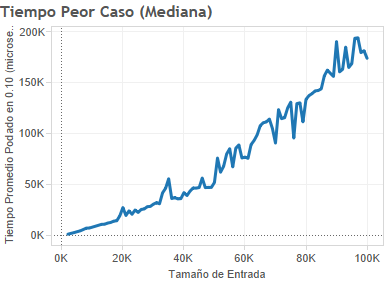
\includegraphics[width=8cm]{images/ex2-worst}
\caption{}
\end{figure}

\ref{grf:ex2-best}

\begin{figure}[h!]
\centering
\label{grf:ex2-best}
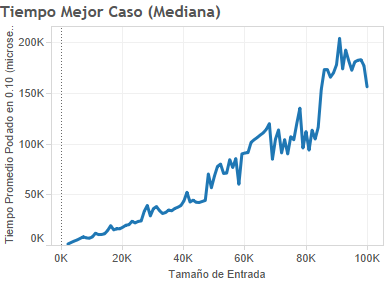
\includegraphics[width=8cm]{images/ex2-best}
\caption{}
\end{figure}

Finalmente, consideramos casos construidos de forma aleatoria, donde el procedimiento consiste en dada una longitud $l$ y una cota máxima $c > 0$ para los números, generar $l$ números aleatoriamente distribuidos en $\{-c, .., c\}$ y ponerlos en una lista. La figura \ref{grf:ex2-random} nos muestra, .

\begin{figure}[h!]
\centering
\label{grf:ex2-random}
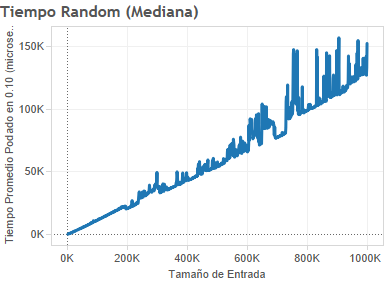
\includegraphics[width=8cm]{images/ex2-random}
\caption{}
\end{figure}

%%% TODOOOOOOOOOOOOO

En conclusión, .

\section{Problema 3}

\subsection{Enunciado}

El capitán de Las Girasoles quiere evitar los problemas en el fogón del año anterior cuando las pequeñas exploradoras rompieron en llanto por no poder sentarse en la ronda junto a sus mejores amigas. En secreto les asignó una letra a cada niña y relevó quién se llevaba con quién.

Su idea es organizar la ronda de manera que exista la menor distancia posible entre cada amistad (Sí, mi querido computador minimizando la suma de las distancias entre todos los pares de amigas).

Resolver en una complejidad estrictamente mejor que $O(e^e a^2)$. Donde $e$ es la cantidad de exploradoras en cada grupo, y $a$ la cantidad de amistades.

\subsection{Resolución y Correctitud}

Resolver el tercer ejercicio requiere de una observación fundamental: todas las formas de sentarse en ronda para las exploradoras son exactamente las permutaciones que podamos formar con ellas. Esto quiere decir que, en concreto, un algoritmo de fuerza bruta para resolver el problema podría simplemente ser generar todas las permutaciones posibles de exploradoras y buscar la mejor según el criterio indicado por la cátedra, de la misma forma en la que buscamos el máximo o el mínimo de un arreglo. Es muy fácil ver que este algoritmo tomaría una complejidad temporal de $\Theta(e! f(e, a))$ con $e$ el numero de exploradoras, $a$ el numero de amistades entre ellas, y $f$ una función que incluye todos los costos adicionales. Si bien siempre que elijamos una secuencia de operaciones relativamente sanas tendríamos que $f(e, a) \in \Theta(e^3 a^2)$, y es intuitivo que el algoritmo resultante cumpliría con la complejidad requerida por la especificación, así como que podemos mejorar la solución aplicando las técnicas que vimos en la materia.

Fundamentalmente, la idea se basa en que podemos utilizar la técnica de backtracking para explorar el espacio de soluciones del algoritmo y encontrar una que cumpla con todos los requisitos. Veremos, también, que podemos optimizar nuestra solución a través de podas en el árbol de estados a explorar, aumentando drásticamente la eficiencia del algoritmo.

Para comenzar, cabe destacar que si tenemos el conjunto de posibles soluciones (es decir, todas las permutaciones) para $e$ exploradoras, es muy fácil construir el conjunto de posibles soluciones para $e+1$ exploradoras: basta con simplemente insertar la exploradora faltante entre medio de todas las que ya tenemos para cada permutación. Más formalmente:

\begin{lemma}
El algoritmo expuesto genera todas las permutaciones de $n$ elementos, a partir de todas las permutaciones de $n-1$ elementos.
\end{lemma}

\begin{proof}
Sea $M_n = \{1, .., n\}$, además, sea $S_n = \{ f : M_n \to M_n / \text{f es biyectiva}\}$ el conjunto de permutaciones $M_n$ elementos. Quiero ver que la función $g : S_n \times M_n \to S_{n+1}$ determinada por

$$g((\sigma_1, .., \sigma_n), k) = (\sigma_1, .., \sigma_{k-1}, n+1, \sigma_k, .., \sigma_n)$$

Es una biyeccion. Veamos que es inyectiva, sean $\sigma, \alpha \in S_n$ y $k, l \in M_n$ tales que

$$g(\sigma, k) = g(\alpha, l)$$

Quiero ver que $k = l \wedge \sigma = \alpha$. Pero observemos que esto implica que

$$(\sigma_1, .., \sigma_{k-1}, n+1, \sigma_k, .., \sigma_n) = (\alpha_1, .., \alpha_{l-1}, n+1, \alpha_l, .., \alpha_n)$$

Es decir, $\sigma_k = n + 1 = \sigma_l$. Como cada elemento aparece una única vez, $k = l$, implicando entonces que $\sigma_i = \alpha_i \forall i \in M_n$, pues de otra forma la igualdad no se cumple.

Veamos ahora que es sobreyectiva, sea $\alpha \in S_{n+1}$, sabemos que $\exists l \in M_{n+1} : \alpha_l = n+1$, tomemos entonces $\sigma = (\alpha_1, .., \alpha_{l-1}, \alpha_{l+1}, .., \alpha_{l+1})$, evaluar $g(\sigma, l)$ da el resultado esperado.

Observemos que la función $g$ es precisamente la que intercala al elemento $n+1$ en la permutación para cada una de las posiciones, implicando que un algoritmo que haga exactamente eso va a generar todas las permutaciones.
\end{proof}

Por lo tanto, tenemos la condición fundamental para crear un algoritmo que realice backtracking, ya que comenzando con una solución vacía podemos generar todos los conjuntos de soluciones incrementalmente hasta llegar al conjunto total de soluciones posibles para la cantidad de exploradoras que deseemos.

Yendo mas lejos, notemos que la semántica adherida por estar considerando rondas implica que las permutaciones que sean rotaciones entre ellas son equivalentes: a modo de ejemplo, las permutaciones $\{(1, 2, 3, 4), (4, 1, 2, 3), (3, 4, 1, 2), (2, 3, 4, 1)\}$ son todas equivalentes miradas como rondas, ya que los extremos están unidos entre si, de forma análoga a las listas circulares. Por lo tanto, podemos intentar evitar generar rotaciones de una permutación.

\begin{definition}
Sean $\sigma, \alpha \in S_n$ permutaciones. Decimos que $\sigma \equiv \alpha \iff$ $\sigma$ y $\alpha$ son rotaciones entre ellas. Observemos que $\equiv$ es una relación de equivalencia, ya que cada una es equivalente a sí misma (por no tener que rotar nada), si una es equivalente con otra, rotar de forma inversa nos da la simetría, y la transitividad es literalmente la suma de rotaciones.

Llamaremos a $\hat{\sigma}$ al representante de la clase de equivalencia a la que pertenece $\sigma$, donde elegimos al mismo como la permutación que sea menor lexicográficamente de todo el conjunto.
\end{definition}

\begin{corollary}
Insertar en las ultimas $n-1$ posiciones no borra soluciones posibles
\end{corollary}

\begin{proof}
Es claro que insertar adelante es lo mismo que insertar al final, ya que como rondas ambas son equivalentes:

$$(i_1, .., i_n, n+1) \equiv (n+1, i_1, .., i_n)$$

Con $i_j$ un ordenamiento arbitrario de los números en $M_n$. Además, $i_1 < n+1$ por lo que la primer alternativa es estrictamente menor lexicográficamente que la segunda, implicando que como solución es mejor (por los parámetros determinados por la cátedra, dado que la suma de distancias entre los pares de amistades se va a preservar) y, por lo tanto, la primer alternativa siempre debería ser elegida antes que la segunda.
\end{proof}

Entonces, podemos explorar el espacio de soluciones en forma de árbol, donde la cabeza es la permutación con un solo elemento, y cada nivel está definido en términos del anterior como aplicar la función $g$ del lema \ref{ej3:generador} a todos los nodos del nivel anterior, utilizando cada uno de los $n-1$ valores más grandes de $M_n$. Observemos, además, que podemos explorar el árbol de forma tal que las permutaciones de menor orden lexicográfico sean exploradas antes, simplemente eligiendo los índices para la inserción de mayor a menor.

\begin{figure}[h!]
\centering
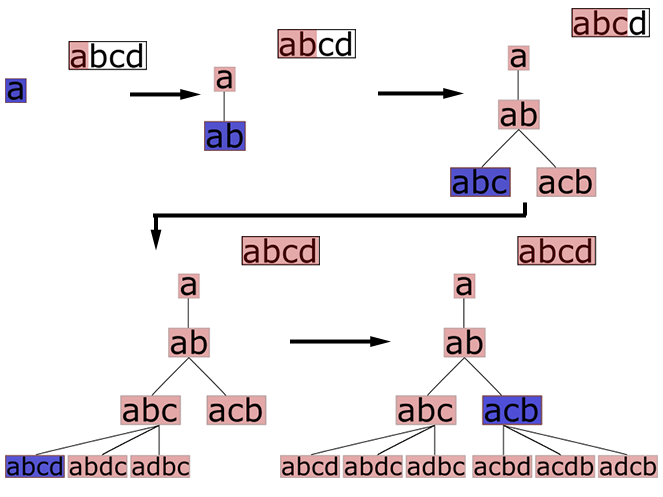
\includegraphics[width=8cm]{images/treeEvolution}
\caption{Ejemplo de generación del espacio de soluciones, en el orden de recorrida, para un caso con exploradoras a, b, c y d.}
\end{figure}

La próxima pregunta natural a realizarse es cual es el tamaño del árbol de búsqueda, que es lo que nos va a permitir estimar la complejidad esperada de nuestra solución:

\begin{lemma}
El árbol de soluciones tiene a lo sumo $(n-1)!$ nodos en cada nivel $n$. Además, cada uno de los nodos en el nivel tiene exactamente $n$ exploradoras.
\end{lemma}

\begin{proof}
Por inducción en el nivel. Cuando $n = 1$, observemos que $(n-1)! = 0! = 1$, y claramente el primer nivel del árbol solo contiene a la permutación $(a)$, por lo que es válido el caso base.

Supongamos que vale para $n$, veamos que vale para $n+1$. Por hipótesis inductiva, los nodos en la frontera son de longitud $n$, y además son en total $(n-1)!$.

Para cada uno de los nodos de la ya explorados, el algoritmo obtiene una de las exploradoras faltantes y la intercala entre cada uno de los índices posibles, comenzando por el $n$-ésimo (el índice $n-1$, ya que estamos indexados desde $0$) y terminando en el índice $1$, por lo que generamos exactamente $n$ nuevos nodos de longitud $n+1$, lo que demuestra la segunda parte del lema.

Además, cada uno de los $(n-1)!$ nodos de la ya explorados tiene exactamente $n$ hijos, y por lo tanto la cantidad de nodos en el nivel $n+1$ es de $(n-1)! n = n! = ((n + 1) - 1)!$; demostrando así la primer parte del lema.
\end{proof}

\begin{corollary}
La cantidad de nodos explorados es $O(e!)$.
\end{corollary}

\begin{proof}
Por el lema anterior, basta con explorar $e$ niveles del árbol, por lo que tenemos que la cantidad de nodos a explorar es, a lo sumo

\begin{equation}
\begin{aligned}
\sum_{i=1}^{e} (i-1)! &= \sum_{i=0}^{e-1} i! \\
&\leq \sum_{i=0}^{e-1} (e-1)! \\
&= (e-1)! (e-1) \in O(e!)
\end{aligned}
\end{equation}

Cabe destacar que, de cualquier forma, las cotas aplicadas en este corolario no son para nada ajustadas, por lo que la cota superior por $e!$ únicamente nos permite demostrar que este algoritmo no es peor que realizar la solución por fuerza bruta.
\end{proof}

\begin{definition}
Si $\sigma \in S_n$, decimos que el tamaño de $\sigma$, notado $|\sigma|$, es $n$.
\end{definition}

\begin{definition}
Dadas $\sigma \in S_n, \alpha \in S_m$ permutaciones, decimos que $\sigma < \alpha$ si $|\sigma| < |\alpha|$ o, en caso de que sean iguales, si la suma de las amistades de $\sigma$ es menor que la de $\alpha$ o, en caso de que estas sean iguales, si $\hat{\sigma} < \hat{\alpha}$ lexicográficamente.
\end{definition}

\begin{definition}
Una permutación es completa cuando la cantidad de elementos de la misma son exactamente la cantidad de exploradoras. Por otro lado, una permutación es parcial cuando es obtenida por el proceso iterativo que describimos anteriormente, y no es completa.
\end{definition}

\begin{lemma}
Dada una permutación completa al problema, cualquier permutación parcial mayor o igual a la permutación dada no va a ser solución del problema.
\end{lemma}

\begin{proof}
Observemos que al insertar un nuevo elemento, la suma de las distancias entre amistades de la solución parcial solo puede aumentar (ya que a lo sumo separamos amistades, pero nunca las juntamos más), llegando entonces a una permutación cuya suma de distancias va a ser mayor estricta que la que ya tenemos, y que por lo tanto no puede ser la solución del problema.
\end{proof}

Es decir, una vez que tenemos una permutación completa generada podemos comenzar a purgar todas las ramas que generen alguna permutación mayor a la que ya tenemos, y esa purga no va a borrar ninguna solución valida. Con esto, tenemos todas las ideas fundamentales para construir nuestro algoritmo de backtracking: comenzando con la solución para una sola exploradora, podemos ir generando las soluciones para cada vez más exploradoras, hasta llegar al final del árbol de estados. Más todavía, podemos comenzar con una primera solución completa al problema, por más mala que sea, y utilizarla como cota superior para purgar ramas del espacio de soluciones, mejorándola a medida que vamos descubriendo nuevas soluciones completas. Pensando en esto, proponemos el siguiente algoritmo como solución al problema:

\begin{algorithmic}[1]
\Procedure{backtracking}{}
\State processing $\gets$ stack vacia \Comment{$O(1)$}
\State inicial $\gets$ ronda vacia asociada al grafo de relaciones \Comment{$O(e)$}
\State processing.push(inicial) \Comment{$O(1)$}
\State inicial $\gets$ alguna solución completa \Comment{$O(e^3 a)$}
\While{processing no esté vacia} \Comment{$O(1)$}
\State actual $\gets$ processing.top() \Comment{$O(1)$}
\State processing.pop() \Comment{$O(1)$}
\If{actual es una solución completa} \Comment{$O(1)$}
\If{actual es mejor solución que inicial} \Comment{$O(e)$}
\State inicial $\gets$ actual \Comment{$O(e)$}
\EndIf
\Else
\For{siguiente in actual.sucesores()} \Comment{$O(e^2 a)$}
\If{no hay que podar el nodo siguiente} \Comment{$O(1)$}
\State processing.push(siguiente) \Comment{$O(1)$}
\EndIf
\EndFor
\EndIf
\EndWhile
\State \textbf{return} inicial
\EndProcedure
\end{algorithmic}

Cabe destacar, esta es una conversión del algoritmo recursivo para hacer backtracking en un algoritmo iterativo.

\subsection{Complejidad}

Para el análisis de complejidad, primero tenemos que aclarar varias cuestiones que surgen a lo largo del código, relacionadas con las estructuras que utilizamos para representar rondas y cómo anda nuestro algoritmo.

Para la representación de las rondas, decidimos utilizar una estructura con redundancia que guarda la permutación que representa, las exploradoras faltantes para completar la ronda, la suma de las distancias entre las amistades, y la máxima distancia entre pares de amistades. Esto nos permite implementar de forma muy simple algunas de las operaciones que más realizamos: ver si una permutación es completa, y obtener alguna exploradora faltante en la permutación. No vamos a realizar el análisis de complejidad de estas operaciones, ya que todas son simples, sin embargo, exponemos en la siguiente tabla las complejidades finales:


\begin{tabular}{c|c}
 Constructor & $O(e)$ \\
 Constructor por Copia & $O(e)$ \\
 Tamaño & $O(1)$ \\
 Insercion & $O(e^2 a)$ \\
 Asignacion & $O(e)$ \\
 Comparacion por menor & $O(e)$ \\
 Verificar si es completa & $O(1)$ \\
 Obtener exploradora faltante & $O(1)$ \\
 Obtener máxima distancia & $O(1)$ \\
 Obtener suma & $O(1)$ \\
 Decidir si podar & $O(1)$ \\
\end{tabular}


\begin{lemma}
El algorítmo es $O(e! e^2 a)$
\end{lemma}

\begin{proof}
Para hacer el análisis de complejidad, vamos a asumir que no tenemos poda, ya que utilizándola a lo sumo mejoramos la complejidad (porque decidir si podar o no es $O(1)$, y por lo tanto no agrega un costo significativo).

Bajo esta suposición, observemos que en todo el árbol tenemos, a lo sumo, $O(e!)$ nodos. Por lo tanto, la cantidad de operaciones que vamos a necesitar realizar es, a lo sumo para cada nodo, el costo de todo lo que hay adentro del while, donde este último es $O(e^2 a)$, y por lo tanto tenemos un total de $O(e! e^2 a)$ operaciones en el peor caso.
\end{proof}

\begin{lemma}
$O(e! e^2 a)$ es estrictamente mejor que $O(e^e a^2)$
\end{lemma}

\begin{proof}
Observemos que

\begin{equation}
\begin{aligned}
\lim_{e \to +\infty} \frac{e! e^2 a}{e^e a^2} &= \frac{1}{a} \lim_{e \to +\infty} \frac{(e-1)!}{e^{e-3}} \\
&= \lim_{e \to +\infty} \frac{\prod_{i=1}^{e-1} i}{e^{e-3}} \\
&= \lim_{e \to +\infty} (\prod_{i=5}^{e-1} \frac{i}{e}) \frac{4}{e} 3 2 1 \\
&\leq \lim_{e \to +\infty} \frac{4}{e} 6 \\
&= 0
\end{aligned}
\end{equation}

Además, claramente ambos elementos del cociente son positivos, por lo que están acotados inferiormente por 0. Es decir, no queda otra más que el límite sea 0 (por la propiedad del sandwich). Por lo tanto, tenemos que $O(e! e^2 a) \subset O(e^e a^2)$ y $O(e^e a^2) \nsubseteq O(e! e^2 a)$, dado que el límite inverso se va a infinito.

Cabe destacar que el menor o igual vale porque si $x \leq e$, $\frac{x}{e} \leq 1$, y cada uno de los factores del producto cumple con la propiedad.
\end{proof}

\subsection{Análisis}

El mejor caso del algoritmo es cuando obtenemos la suma óptima lo antes posible, ya que nos va a permitir podar la mayor cantidad de nodos en total. En nuestro caso, como la primer suma calculada se corresponde con la ronda $(z..a)$, por lo que tenemos que pedir que el representante de la clase de equivalencia ($(a z .. b)$) a la que pertenece la misma sea el óptimo (ya que esto nos va a permitir purgar la mayor cantidad de ramas posibles). Observando la figura \ref{grf:ex3-worst}

\begin{figure}[h!]
\centering
\label{grf:ex3-worst}
\includegraphics[width=8cm]{images/ex3-worst}
\caption{}
\end{figure}

En términos del peor caso, es claro darse cuenta que el mismo será cuando la poda sea mínima, es decir, cuando jamás logremos podar nodos. Observemos que esto se corresponde con que las rondas que vayan avanzando lexicográficamente vayan al mismo tiempo bajando el costo, por lo que es difícil poder construir explícitamente un peor caso. Sin embargo, podemos aproximarnos si consideramos no podar el árbol: borrar las podas se correspondería con un caso lo suficientemente malo como para que las mismas sean inaplicables. Si bien esto difícilmente suceda en un caso real, ya que al tener aunque sea un caso muy posiblemente logremos borrar algunas ramas, pensamos que es una buena forma de cuantificar cuánto estamos ganando con las podas. Como se ve en la figura \ref{grf:ex3-best}

\begin{figure}[h!]
\centering
\label{grf:ex3-best}
\includegraphics[width=8cm]{images/ex3-best}
\caption{}
\end{figure}

Finalmente, consideramos casos construidos de forma aleatoria, donde el procedimiento consiste en dada una cantidad de exploradoras $e$ y una cantidad de amistades $a \in \{1, .., \frac{e(e-1)}{2}\}$, generamos el producto cartesiano entre las exploradoras, filtramos los vértices inadmisibles (la relación diagonal y los simétricos), y tomamos una muestra de $a$ elementos uniformemente distribuidos entre los mismos. Como podemos ver en la figura \ref{grf:ex3-random}

\begin{figure}[h!]
\centering
\label{grf:ex3-random}
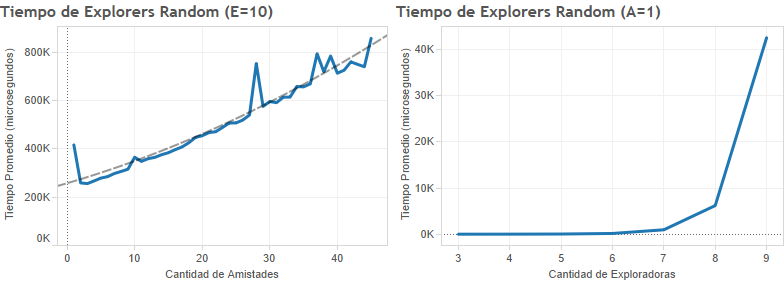
\includegraphics[width=8cm]{images/ex3-random}
\caption{}
\end{figure}

%%% TODOOOOOOOOOOOOO

En conclusión, .

\section{Código fuente}

\end{document}